\documentclass[margin=0.5mm]{standalone}
\usepackage{pgfplots}
\usetikzlibrary{pgfplots.groupplots}
\pgfplotsset{compat=1.7}

\definecolor{BoxCol}{rgb}{0.43,0.62,0.86}
%\definecolor{BoxCol}{rgb}{0.5686,0.07451,0.07451}
%\definecolor{BoxCol}{RGB}{62,126,148}
\begin{document}
	\thispagestyle{empty}
%	\begin{figure}[t]
%		\centering
		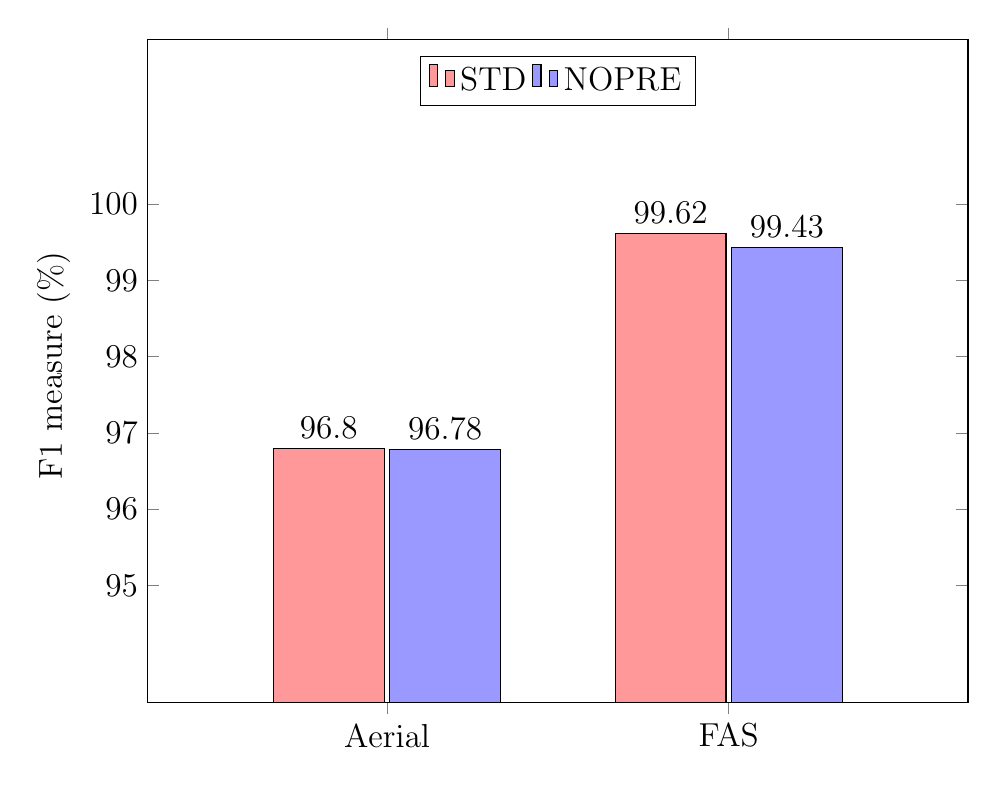
\begin{tikzpicture}
		\begin{axis}[
		width=12cm,
		height=10cm,
		ybar,
		enlargelimits=0.70,
		legend style={at={(0.5,0.975)},
		anchor=north,legend columns=-1},
		ylabel={\ F1 measure (\%)},
		symbolic x coords={Aerial,FAS,NOPRELP},
		xtick=data,
		nodes near coords,
		nodes near coords align={vertical},
		bar width=40pt,
		style={font=\large},
		ytick={95,96,...,100},
%		ymax=100,
		ymin=96
		]
%					STD		NPRE
%			Aerial	96.80	96.78
%			FAS		99.62	99.43
			
%		\addplot [color=black,fill=darkgray] coordinates {(Aerial,96.80) (FAS,99.62) };
%		\addplot [color=black,fill=lightgray] coordinates {(Aerial,96.78) (FAS,99.43) };
		%withcolor
		\addplot [color=black,fill=red!40!white] coordinates {(Aerial,96.80) (FAS,99.62) };
		\addplot [color=black,fill=blue!40!white] coordinates {(Aerial,96.78) (FAS,99.43) };		
		\legend{STD,NOPRE}
		\end{axis}
		\end{tikzpicture}
		%\vspace{-0.7cm}
		%\caption{Left: the pitch distribution for the 10 male speakers. Right: the active speech level for the 20 speakers.}\label{fig:pitch}
		%\vspace{-0.5cm}
%	\end{figure}
\end{document}